\section{eo\-Fl\-Or\-KMutation$<$ EOT $>$ Class Template Reference}
\label{classeo_fl_or_k_mutation}\index{eoFlOrKMutation@{eoFlOrKMutation}}
Applies an atomic mutation to a fixed number of components (1 by default).  


{\tt \#include $<$eo\-Fl\-Or\-Mon\-Op.h$>$}

Inheritance diagram for eo\-Fl\-Or\-KMutation$<$ EOT $>$::\begin{figure}[H]
\begin{center}
\leavevmode
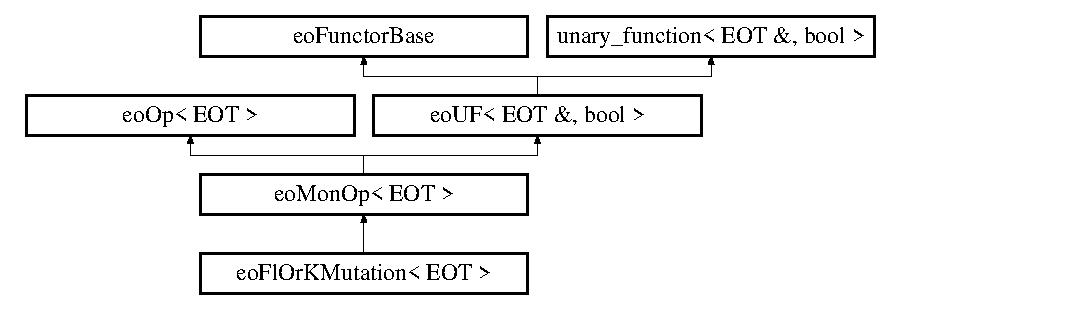
\includegraphics[height=3.71476cm]{classeo_fl_or_k_mutation}
\end{center}
\end{figure}
\subsection*{Public Types}
\begin{CompactItemize}
\item 
typedef EOT::Atom\-Type {\bf Atom\-Type}\label{classeo_fl_or_k_mutation_w0}

\end{CompactItemize}
\subsection*{Public Member Functions}
\begin{CompactItemize}
\item 
{\bf eo\-Fl\-Or\-KMutation} ({\bf eo\-Mon\-Op}$<$ Atom\-Type $>$ \&\_\-atom\-Mutation, unsigned \_\-nb=1)\label{classeo_fl_or_k_mutation_a0}

\begin{CompactList}\small\item\em default ctor: requires an Atom mutation \item\end{CompactList}\item 
bool {\bf operator()} ({\bf EOT} \&\_\-eo)\label{classeo_fl_or_k_mutation_a1}

\begin{CompactList}\small\item\em applies the atom mutation to K randomly selected components \item\end{CompactList}\item 
virtual std::string {\bf class\-Name} () const \label{classeo_fl_or_k_mutation_a2}

\begin{CompactList}\small\item\em inherited {\bf class\-Name()}{\rm (p.\,\pageref{classeo_fl_or_k_mutation_a2})} \item\end{CompactList}\end{CompactItemize}
\subsection*{Private Attributes}
\begin{CompactItemize}
\item 
unsigned {\bf nb}\label{classeo_fl_or_k_mutation_r0}

\item 
{\bf eo\-Mon\-Op}$<$ Atom\-Type $>$ \& {\bf atom\-Mutation}\label{classeo_fl_or_k_mutation_r1}

\end{CompactItemize}


\subsection{Detailed Description}
\subsubsection*{template$<$class EOT$>$ class eo\-Fl\-Or\-KMutation$<$ EOT $>$}

Applies an atomic mutation to a fixed number of components (1 by default). 



Definition at line 82 of file eo\-Fl\-Or\-Mon\-Op.h.

The documentation for this class was generated from the following file:\begin{CompactItemize}
\item 
eo\-Fl\-Or\-Mon\-Op.h\end{CompactItemize}
